\documentclass[12pt,a4paper]{article}
\usepackage[utf8]{inputenc}
\usepackage[spanish]{babel}
\usepackage[margin=0.5in, top=0.5in, bottom=0.5in]{geometry}
\usepackage{amsmath}
\usepackage{amsfonts}
\usepackage{amssymb}
\usepackage{hyperref}
\usepackage[shortlabels]{enumitem}
\usepackage{graphicx}
\newcommand{\p}{\phantom{......}}

\usepackage{setspace}
\onehalfspacing

\title{Bases de datos 2023-1\\
Tarea 3: Modelo Relacional}
\begin{document}
\maketitle

\begin{enumerate}
	\item Preguntas de repaso.
		\begin{enumerate}
			\item[\textbf{i.}] ¿Qué es una relación y qué características tiene?\\

				Es un subconjunto del producto cartesiano de otros conjuntos (dominios).
				Cada elemento del subconjunto representa una entidad y cada entrada de los
				elementos es una pieza de información de la entidad.

				Las relaciones tienen:

				\textbf{Nombre}: Las identifica de otras relaciones.\\
				\textbf{tuplas}: Elementos de la relación, cada una representa una entidad.\\
				\textbf{atributos}: Elementos de las tuplas que describen propiedades de sus entidades.\\
				\textbf{Dominios}: Los conjuntos a los que pertenecen los atributos, en la entrada $x$
				de una tupla siempre hay elementos del mismo dominio.\\
				\textbf{Cardinalidad}: La cantidad de tuplas en una relación.\\
				\textbf{Grado}: La cantidad de entradas en la tupla (cantidad de atributos).\\
				\textbf{Restricciones}: Estructuras que no se permiten en una relación.\\	


			\item[\textbf{ii.}] ¿Qué restricciones impone una llave primaria y
				una llave foránea al modelo de datos relacional?\\

				\textbf{Primaria}: Unicidad. No pueden existir dos tuplas con los mismo valores
				en los atributos que componen sus llaves primarias.\\

				\textbf{Foránea}: Identificación y existencia. Debe de existir una entidad
				en otra relación que tenga como llave primaria esta llave foránea.\\


				\pagebreak
			\item[\textbf{iii.}] Investiga que cuáles son las Reglas de Codd y explica con tus propias palabras
				cada una de ellas. Indica por qué consideras que son importantes.\\

				\begin{enumerate}
					\item[0.] Todo sistema de manejo de bases de datos relacionales,
						debe manejar sus bases de datos usando solo relaciones.\\

						Toda la información de las bases de datos está en tablas.\\

					\item[1.] Toda la información de una base de datos relacional se
						representa como valores en tablas.\\

						La información de la base de datos se accesa con tablas.\\

					\item[2.] Todos los datos en una base de datos relacional se deben
						de poder acceder usando solo el nombre de la tabla, una llave primaria
						y el nombre de una columna.\\

						Para extraer un dato único de una base de datos solo se necesita saber
						en que tabla está, a que entidad pertenece y de que columna es.
						Esta regla también impide los valores multivaluados.\\

					\item[3.] Los valores nulos deben ser soportados y representan información
						faltante o inexistente independientemente de un tipo de dato.\\

						Todos los lugares donde puede haber datos también pueden tener null,
						para representar que no hay o no puede haber un dato para esa entrada
						de la tabla.\\

					\item[4.] La descripción de la base de datos se representa en el nivel
						lógico de la misma forma que datos normales para que pueda ser
						manipulada con el mismo lenguaje relacional que ocupan los datos normales.\\

						Debe de haber un catálogo y este debe de poderse modificar con
						el mismo lenguaje que el resto de la base. Esto hace cómodo
						manipular muchas bases de datos al mismo tiempo (entre otras cosas).\\

					\item[5.] Un sistema relacional puede soportar más lenguajes e interfaces, pero
						debe haber almenos uno con expresiones bien definidas en texto y que pueda:
						\{definir datos, ver definiciones, manipular datos, restringir integridad,
						controlar autorización, definir transacciones\}.\\

						Básicamente dice que además de todos los extras que tenga un sistema
						manejador relacional, este debe de poder aceptar ``comandos''
						para todas sus operaciones.\\

						\pagebreak
					\item[6.] Todas las vistas que se pueden actualizar en teoría pueden
						ser actualizadas por el sistema.\\

						El sistema puede actualizar las tablas de las que dependen
						las vistas si estas en el modelo lógico se pueden actualizar
						sin problemas.\\

					\item[7.] La capacidad de manejar una relación como operando aplica para
						la inserción, actualización y eliminación de los datos.\\

						Insertar, actualizar y eliminar datos de la base se debe poder
						hacer para colecciones de entidades de una relación al mismo tiempo.\\

					\item[8.] Aplicaciones y servicios no son afectados lógicamente cuando
						se cambia el almacenamiento o la forma de acceder a este.\\

						La base de datos no debe ser afectada cuando se mueven los datos,
						se cambia su mecanismo de almacenamiento o se distribuyen.\\

					\item[9.] Aplicaciones y servicios no son afectadas cuando cambios
						que no alteran la información se hacen en las tablas.\\

						La interfase entre las aplicaciones y el sistema manejador
						debe de ser independiente de la estructura de las tablas.\\

					\item[10.] Las restricciones de integridad se deben de poder definir en
						el lenguaje de la base de datos y almacenar en el catálogo, no
						en las aplicaciones o servicios que usen la base.\\

						Las restricciones son resguardadas por el sistema de base de datos,
						por ejemplo, la unicidad de las llaves primarias nos la debe
						de asegurar el sistema, no las aplicaciones que hagan interfaces
						con él.\\

					\item[11.] Un sistema manejador de bases de datos relacionales, tiene
						independencia a la distribución.\\

						Estos sistemas deben de comportarse de la misma manera si importar
						como esta distribuida su información en una red (una sola instancia, muchas).\\

					\item[12.] Si un sistema manejador tiene un lenguaje de bajo nivel,
						este no debe de poder ignorar las restricciones impuestas en
						otro lenguaje de alto nivel.\\

						La intención es que las restricciones puedan ser aseguradas
						en el sistema, que de verdad sean invariantes sin importar
						como se accesa el sistema.\\
				\end{enumerate}

				Son importantes por que limitan lo que puede ser considerado como base de datos relacional.
				Homogenizan los SMDBR para simplificar como son usados por los programas o usuarios.
				También aseguran las necesidades básicas de estos sistemas, lo que es necesario
				para poder utilizarlos eficazmente.\\

				(fuente: \url{https://reldb.org/c/index.php/twelve-rules/} recuperado en 2022-10-03).\\
		\end{enumerate}

	\item Modelo Relacional.
		\begin{enumerate}
			\item[a.] Traduce el siguiente modelo Entidad – Relación a su correspondiente Modelo Relacional.

				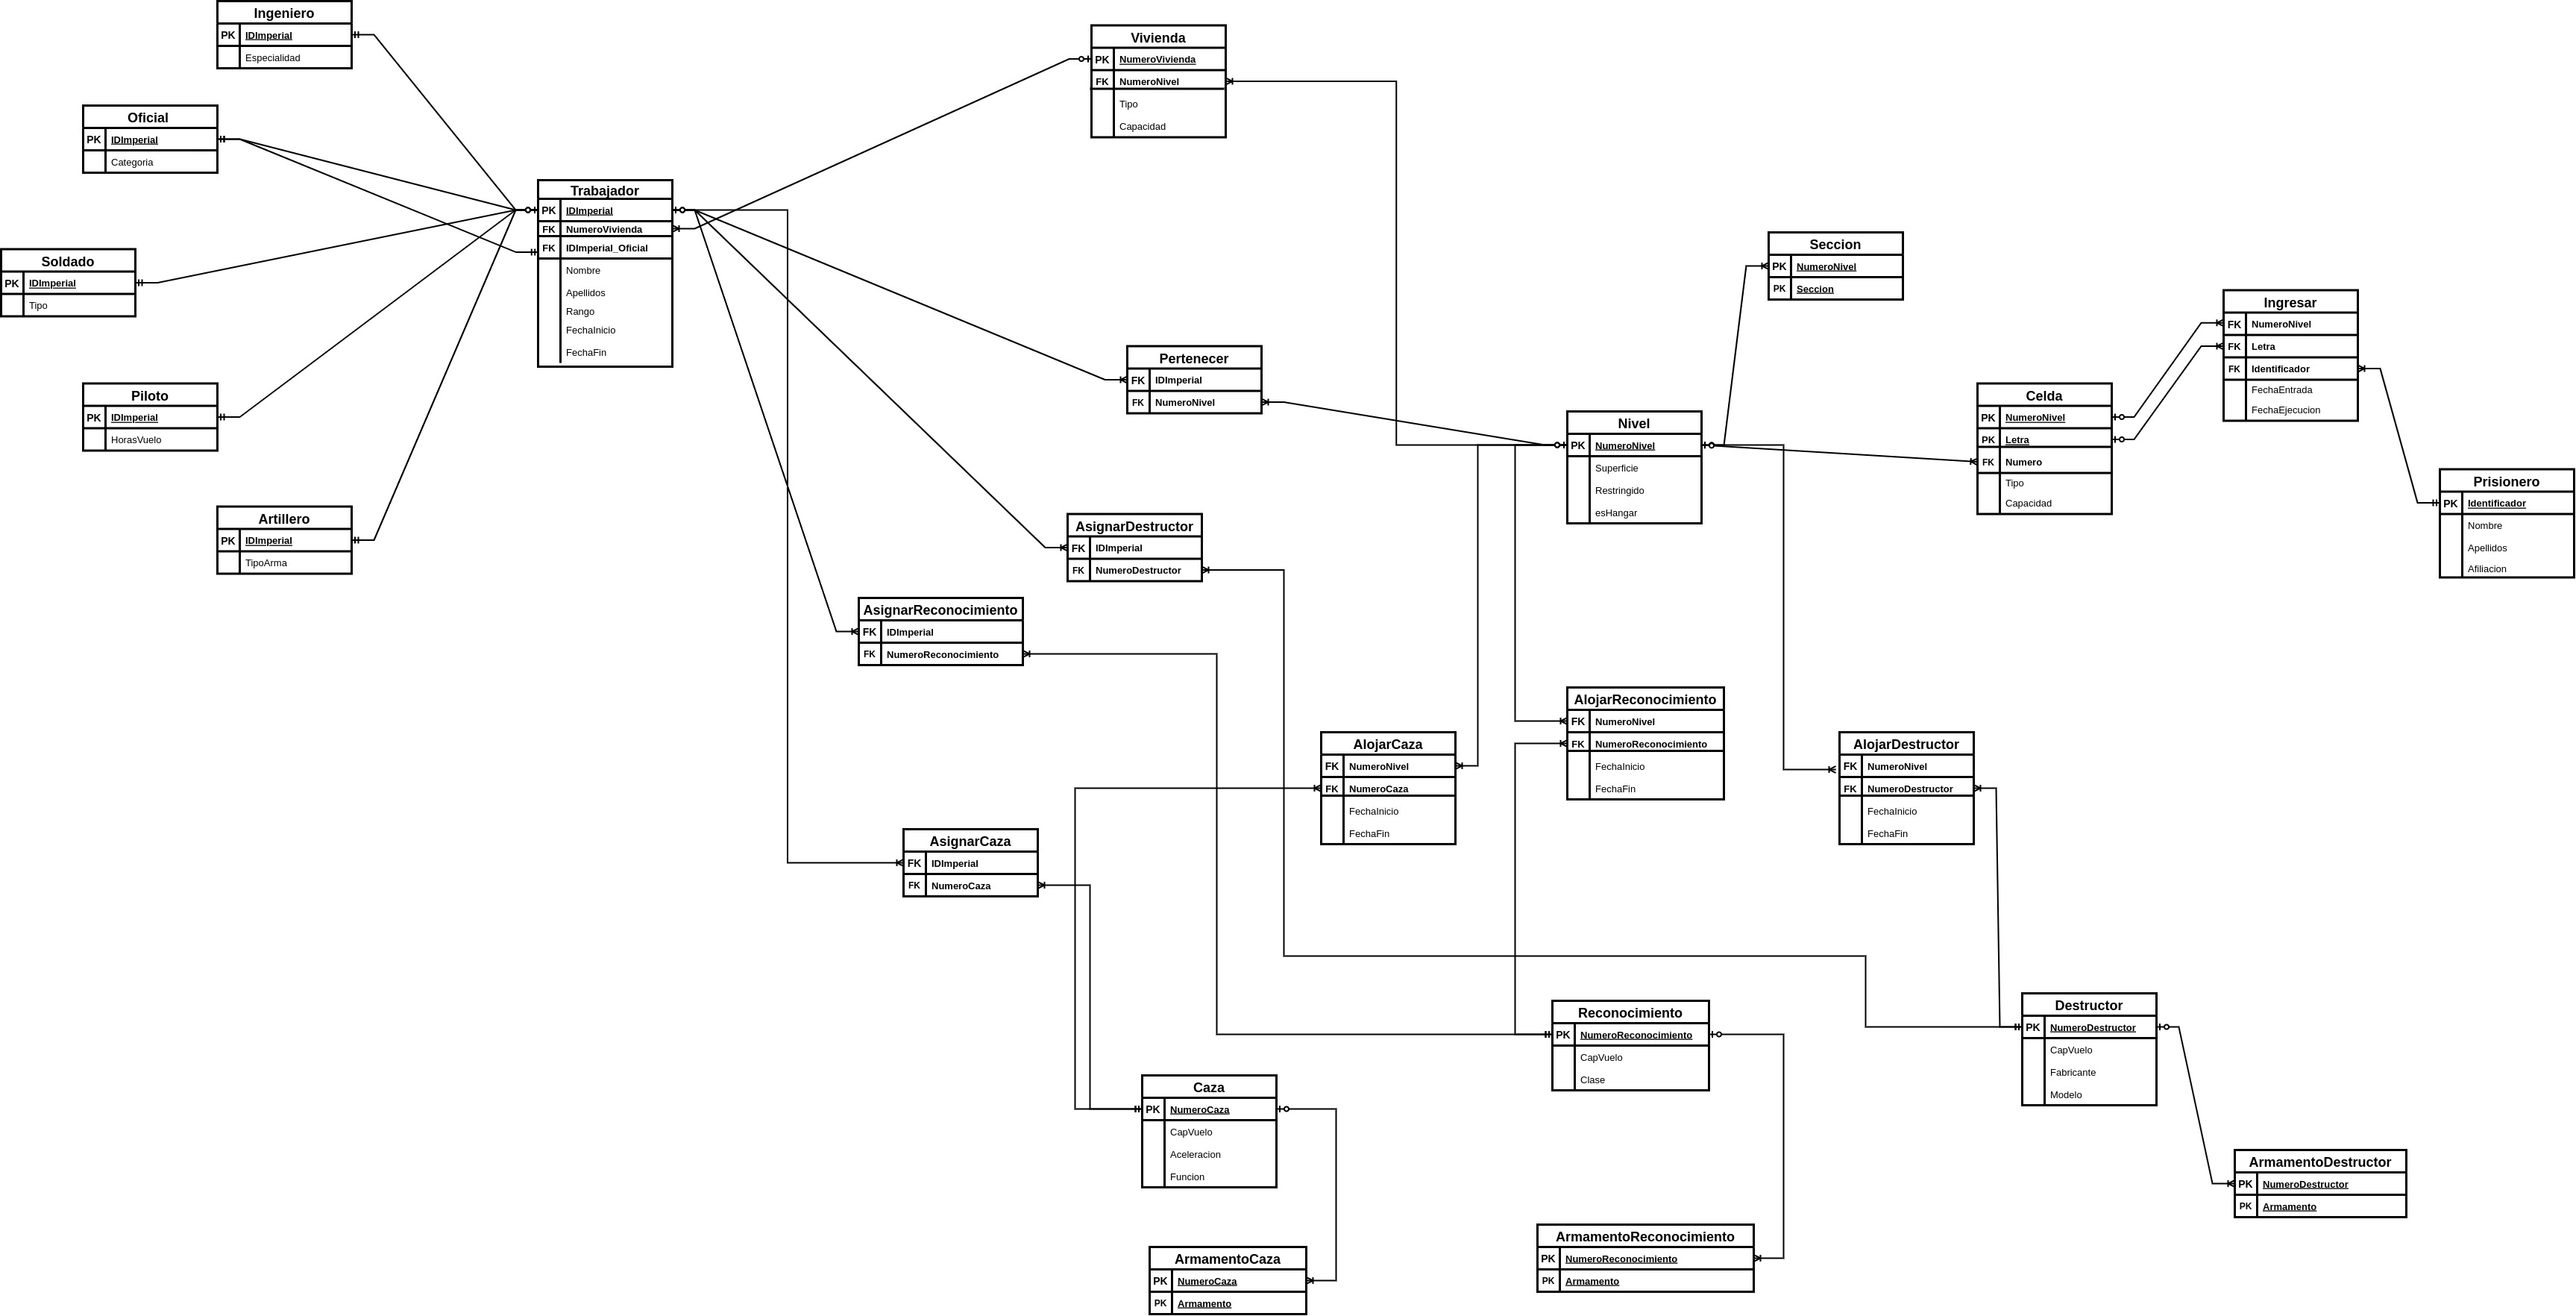
\includegraphics[scale=0.1]{../Diagramas/Ejercicio2a.jpg}

Se cambio el nombre del atributo ``Numero''  por un nombre mas especifico para mejorar la lectura en el modelo relacional, por ejemplo para la Vivienda se eligió ``NumeroVivienda'', esto con cada tabla que tuviera como PK ``Numero''.
En el caso de la tabla Celda, dado que ya teníamos el nombre NumeroNivel como su PK (pues Celda es una entidad débil con respecto a Nivel), al Nivel mandarle como FK su PK (dado que Tener es una relacion débil con atributos, esta deber ser manejada como el caso de una relacion 1:M) decidimos cambiar el nombre por solamente Numero.
		\end{enumerate}

		\pagebreak
	\item Modelo Relacional e inserción de tuplas.

		Considera el siguiente Modelo E/R:

		\begin{enumerate}
			\item[a.] Completa la tabla que se presenta a continuación, convirtiendo el Modelo E-R
				en un Modelo Relacional, para todas las opciones de cardinalidad
				(considera en todos los casos, participación parcial).
				Indica las relaciones resultantes, su llave primaria y la integridad referencial.

				\begin{tabular}{|l|l|}
					\hline
					Modelo E-R	&	Modelo Relacional\\
					\hline
					M:N			&	A(\underline{a1}, \underline{a2}, a3)
					            		&&  B(\underline{b}, b1)
			       			                &&  ab(a1, a2, b, ab1)\\
					\hline
					1:N			&	A(\underline{a1}, \underline{a2}, a3)
							        &&  B(\underline{b}, a1, a2, ab1, b1)\\
					\hline
					N:1			&	A(\underline{a1}, \underline{a2}, b, ab1, a3)
						       	   	&&  B(\underline{b}, b1)\\
					\hline
					1:1			&	A(\underline{a1}, \underline{a2}, a3)
							        &&  B(\underline{b}, b1)
							        &&  ab(a1, a2, b, ab1)\\
					\hline
				\end{tabular}

				\pagebreak
			\item[b.] Del inciso a) toma el MR que obtuviste para la cardinalidad M : N.
				Asume que los atributos a1, b y ab1 son de tipo entero, mientras que a2, a3 y b1 son de tipo cadena.
				Supón que la relación A tiene 4 tuplas con los siguientes valores
				(2,’ww’,’a’), (4,’xx’,’b’), (6,’yy’,’c’), (8,’zz’,’d’) y la relación B tiene 5
				tuplas identificadas por los valores 17, 27, 37, 47, 57.
				Los incisos que se presentan a continuación, representan un conjunto de tuplas a
				insertar (en ese orden) en la relación AB, indica cuál conjunto se puede insertar
				completamente en dicha relación. Justifica tu respuesta en cada caso.

				\begin{enumerate}
					\item[i.] (8,’zz’,17,5); (6,’yy’,57,10); (4,’xx’,27,15); (2,’ww’,37,20); (4,’xx’,27,15)\\
					\item[ii.] (17,’zz’,2,’m’); (27,’yy’,4,’n’); (37,’xx’,6,’o’); (47,’ww’,8,’p’); (57,’zz’,4,’q’)\\
					\item[iii.] (2,’a’,17,23); (4,’b’,27,24); (6,’c’,37,25); (8,’d’,47,26); (2,’a’,57,27)\\
					\item[iv.] (2,’ww’,57,’a’); (4,’xx’,37,’a’); (6,’yy’,17,’a’); (8,’zz’,17,’a’); (10,’xx’,27,’a’)\\
				\end{enumerate}
				
				\textbf{Respuesta}\\
				Los conjuntos ii. y iv. quedan descartados ya que los atributos de ab son a1, a2, b, y ab1 (entero, cadena, entero y entero respectivamente). Es decir, tenemos tres atributos de tipo entero y uno de tipo cadena, y las tuplas indicadas en estos incisos no cumplen con estas características de tener 3 entradas enteras y una de cadena.\\

				Respecto a los otros dos conjuntos, podríamos descartar alguno si suponemos cuál es el atributo que corresponde exactamente a a2.
				Es decir, tomando como ejemplo a la tupla de A, (2,'ww','a'), si suponemos que 'ww' corresponde al atributo a2 (es decir que 'ww' funciona como llave de la tupla), entonces podríamos estar tentados a decir que la respuesta sería el inciso i. Sin embargo observemos que hay una tupla repetida, (4,'xx',27,25), por lo que este inciso no es un conjunto y a nosotros se nos pide seleccionar algún conjunto de i. ii. iii. y iv., por lo que descartaremos este inciso (además de que se nos pide \textbf{insertar} completamente el conjunto, que si lo viéramos como conjunto tendríamos que decir que son cuatro tuplas en total, y en este caso sí lo podríamos insertar totalmente, pero si lo que queremos es insertar dos tuplas iguales, esto no se permitiría porque serían datos redundantes).\\

				Por lo que tendremos que suponer que, dentro del mismo ejemplo con la tupla de A, 'a' es el valor que corresponde al atributo a2 de la tupla. Entonces la respuesta sería el inciso iii. ya que para insertar tuplas en la relación ab necesitamos la llave primaria de la tupla de A y de la tupla de B, la de B la tenemos en la tercera entrada de las tuplas (es decir, 17, 27, 37, 47, 57) y las llaves de A también (2 y 'a', 4 y 'b', 6 y 'c', 8 y 'd').\\


				\pagebreak
			\item[c.] Del inciso a) toma como base el MR que obtuviste para la cardinalidad 1 : N.
				Los incisos que se presentan a continuación representan un conjunto de tuplas a insertar
				(en ese orden) en la relación B, indica cuál conjunto se puede insertar completamente
				en dicha relación. Justifica tu respuesta en cada caso.

				\begin{enumerate}
					\item[i.] (2,’f’,57,’zz’); (4,’g’,47,’yy’); (6,’h’,37,’xx’); (8,’i’,27,’ww’); (2,’j’,17,’yy’)\\
					\item[ii.] (17,’ww’); (27,’xx’); (37,’yy’); (47,’zz’); (57,’zz’); (17,’xx’); (27,’yy’)\\
					\item[iii.] (57,’f’,8,’zz’); (47,’g’,6,’yy’); (37,’h’,4,’xx’); (27,’i’,2,’ww’); (17,’j’,6,’yy’)\\
					\item[iv.] (57,’f’,8,’a’); (47,’g’,6,’b’); (37,’h’,4,’c’); (27,’i’,2,’d’); (17,’j’,6,’c’)\\
				\end{enumerate}
				
				\textbf{Respuesta}\\
				Analizaremos uno a uno los incisos, y tendremos en cuenta 3 cosas en todos. La primera es que para insertar una tupla en la tabla de B el único atributo necesario en todas las tuplas es b, su llave primaria de dominio entero. \\
				En segundo lugar, que para insertar una tupla en B que no esté relacionada con alguna tupla de A (o sea que tenga valor nulo en las llaves foráneas a1 y a2), el máximo número de atributos es dos. Es decir, una tupla no relacionada con otra de A se tendría que ver como (b, b1) como máximo, mientras que para insertar una tupla que \textbf{sí} esté relacionada con otra de A (o sea, que tenga valores no nulos en las llaves foráneas a1 y a2), el mínimo y máximo número de atributos que puede tener dicha tupla de B son 3 y 5 respectivamente, es decir que algunas tuplas de B se pueden ver como (b, a1, a2), también como (b, a1, a2, ab1), como (b, a1, a2, b1) y como (b, a1, a2, ab1, b1). Una consecuencia de esto es que una tupla de B de tres o más atributos necesariamente debe estar relacionada con alguna de A.\\

				Y en tercer lugar que supondremos que la tabla de B está vacía y que la tabla de A contiene únicamente las tuplas que se especificaron en el inciso b).\\

				\textbf{i.} No se pueden insertar estas tuplas porque tienen más de tres atributos, lo que significa que al menos los valores de los atributos a1 y a2 son no nulos, entonces estos atributos en conjunto deben representar una llave primaria en la tabla de A. Tomando como ejemplo la primera tupla, (2, 'f', 57, 'zz'), ninguna combinación de entero-cadena representa una llave primaria en la tabla de A. Por ejemplo ni (2, 'f') ni (2, 'zz') son llaves primarias en la tabla de A.\\

				\textbf{ii.} No se puede insertar este conjunto en su totalidad. Una de las razones es porque, como intentamos intentar las tuplas en el orden presentado, podremos insertar la tupla (17, 'ww') ya que está en la forma de los dominios de (b, b1), sin embargo cuando lleguemos a la tupla (17, 'xx') no podremos insertar ambas tuplas al mismo tiempo porque no podemos tener llaves primarias repetidas.\\

				\textbf{iii.} Estas tuplas sí podemos insertarlas bajo una suposición extra. Como estamos suponiendo que la tabla de A está llena como nos indica el inciso b) y en este no se especifica si los valores 'ww', ... , 'zz' corresponden al atributo a2 o al atributo a3, si suponemos que corresponden a a2, entonces sí podemos insertar las tuplas porque todas cumplen estar en el formato (b, b1, a1, a2) $\sim$ (entero, cadena, entero, cadena) \\

				\textbf{iv.} Este conjunto no se puede insertar, ya que aunque como en el conjunto anterior, las tuplas están en un formato válido para la inserción en B respecto a los dominios ((entero, cadena, entero, cadena)), como hay más de 3 atributos, necesariamente debe haber llaves para una tupla de A, y en ninguna tupla de este conjunto las hay (aún si supusiéramos que las llaves de A correspondientes a a2 son 'a', 'b', 'c'. 'd'), en particular en la primera tupla no hay ninguna combinación entero-cadena que cumpla ser llave de una tupla válida de A. Por ejemplo (8, 'a'), (8, 'f') no es llave de ninguna tupla de A.\\


			\item[d.] Considera el mismo escenario del inciso b para las relaciones A y B.
				Toma como base el Modelo Relacional que obtuviste para la cardinalidad 1:1.
				Supón que tu modelo tiene participación total del lado de la relación A.
				Propón un conjunto de 4 tuplas que se pueda insertar en A y un conjunto que no se pueda insertar
				(también de 4 tuplas). Justifica tu respuesta en cada caso.
				
				\textbf{Respuesta}\\
			    Si suponemos que hay participación total del lado de A, entonces el modelo relacional cambia. Las tablas de A y B quedarían de la siguiente manera:\\
			    A(\underline{a1}, \underline{a2}, b, a3, ab1)\\
				B(\underline{b}, b1)\\\\
				Entonces el conjunto de 4 tuplas que sí se puede insertar en A que proponemos es:\\
				(1, 'e', 17); (3, 'f', 27); (5, 'g', 37); (7, 'h', 47)\\
				todas en formato (a1, a2, b) y con los atributos correspondientes a a3 y ab1 con valor nulo. Estas se pueden insertar ya que tienen llave primaria de una tupla que no existe en A, además de que como A está obligada a relacionarse con B por la participación total, todas tienen asignada una llave de alguna tupla de B, y como todas estas llaves de B son diferentes para cada tupla también cumplen con la cardinalidad 1:1.\\

				Mientras que el conjunto de 4 tuplas que no se puede insertar que proponemos es:\\
				(1); (2); (3); (4)\\

				No se pueden insertar porque en particular la primera tupla de estas no se puede insertar ya que ni siquiera cuenta con llave primaria, porque la llave primaria de todas las tuplas de A deben constar de un entero y una cadena y en este caso sólo tenemos un entero.
		\end{enumerate}

		\pagebreak
	\item Modelo Relacional y restricciones de integridad.\\

		A continuación, se encuentra el Modelo Relacional de un departamento de recursos humanos de alguna empresa.
		En este esquema, supón que desde es inclusivo, mientras que hasta es exclusivo,
		definiendo el período [desde,hasta).
		Indica cuáles de las siguientes afirmaciones se cumplen y por qué razón
		(sin considerar restricciones adicionales):

		\begin{enumerate}
            \item[a.] Dos departamentos con el nombre ‘Sistemas’ podrían existir al mismo tiempo.\\
            
            Si, pues el nombre del departamento no actúa como Primary Key, así que se puede repetir.\\
            
            \item[b.] Dos o más empleados pueden administrar el mismo Departamento al mismo tiempo.\\
            
            Si, pues la cardinalidad entre Empleado y Administrar es uno opcional a muchos obligatorios y la cardinalidad entre Empleado y Departamento es muchos obligatorio a uno opcional, por lo que tenemos que varios empleados pueden administrar varios departamentos. \\
            
            \item[c.] Un empleado puede trabajar en un Departamento y administrar otro al mismo tiempo.\\
            
            Si. Las cardinalidades de Trabajar son iguales a las de Administrar. Por lo tanto tenemos que varios empleados pueden trabajar en varios departamentos, y varios empleados pueden administrar varios departamentos. \\
            
            \item[d.] Para administrar un Departamento un empleado debe trabajar en dicho departamento.\\
            
            No, las relaciones de Trabajar y Administrar son separadas, y nada impide que una persona administre un Departamento sin trabajar en él. \\
            
            \item[e.] Un empleado podría trabajar en dos Departamentos a partir de la misma fecha.\\
            
            Si, pues aunque Desde es Primary Key, también NúmDepto y NúmEmpleado Primary Key, por lo que no es necesario que Desde sea individualmente única, solo se requiere que las 3 en conjunto sean únicas.\\
            
            \item[f.] Para las tuplas de la relación Administrar, hasta no puede ser anterior a desde.\\
            
            No. Aunque es evidente que esto no se debería permitir, el esquema por sí solo no impone esta restricción.\\
            
			\pagebreak
            \item[g.] Dado un empleado, podemos identificar exactamente el Departamento donde trabaja.\\
            
            Si*, basta ver en Trabajar todas las tuplas que tengan en NúmEmpleado el mismo valor que el NúmEmpleado de nuestro Empleado y los departamentos que compartan NúmDepto con el NúmDepto de dichas tuplas, y así podemos identificar los departamentos en los que trabaja dicho Empleado. \\
            *Si se pueden identificar los departamentos en los que trabaja, pero no podemos asegurar que es un solo departamento.\\
            
            \item[h.] Ningún empleado puede cobrar más de un Salario al mismo tiempo.\\
        
            No, la cardinalidad entre Empleado y Salario es 1 opcional a muchos obligatoria, y aunque la fecha de inicio tiene que ser única para cada NúmEmpleado, nada impide que se inicie otro salario antes de que termine el anterior. \\
            
            \item[i.] Algunas tuplas en Salario podrían no tener valor para el atributo desde
                y ningún empleado asociado a ellas.\\
            
            No. Por un lado, la cardinalidad entre Empleado y Salario es 1 opcional a muchos obligatoria, por lo que todas las tuplas en Salario deben obligatoriamente tener un empleado. Por otro lado, ya que Desde es Primary Key, no puede haber tuplas que no contengan este valor.\\
                
            \item[j.] Un Departamento siempre tiene algún empleado que lo administre\\
            
            No, pues la cardinalidad entre Departamento y Administrar es 1 opcional a muchos obligatorio, por lo tanto puede haber Departamentos que no son administrados por ningún Empleado.\\
        
        \end{enumerate}

\end{enumerate}
\end{document}
